% =============================================================================
% Learned Heuristics for the Asymmetric Traveling Salesman Problem
% on Real Road Networks
% =============================================================================
\documentclass[11pt,a4paper]{article}

% ---------- packages ----------
\usepackage[margin=1in]{geometry}
\usepackage{amsmath,amssymb,amsfonts}
\usepackage{algorithm}
\usepackage{algorithmic}
\usepackage{booktabs}
\usepackage[colorlinks=true,citecolor=blue,linkcolor=blue,urlcolor=blue]{hyperref}
\usepackage[round]{natbib}
\usepackage{pgfplots}
\pgfplotsset{compat=1.17}
\usepackage{tikz}
\usetikzlibrary{positioning,arrows.meta,shapes.geometric,fit,calc,decorations.pathreplacing}
\usepackage{subcaption}
\usepackage{multirow}
\usepackage{xcolor}
\usepackage{graphicx}
\usepackage{enumitem}
\usepackage{array}

% ---------- custom colors ----------
\definecolor{deepblue}{HTML}{1f77b4}
\definecolor{deeporange}{HTML}{ff7f0e}
\definecolor{deepgreen}{HTML}{2ca02c}
\definecolor{deepred}{HTML}{d62728}
\definecolor{deeppurple}{HTML}{9467bd}

% ---------- custom commands ----------
\newcommand{\ie}{\textit{i.e.}}
\newcommand{\eg}{\textit{e.g.}}
\newcommand{\etal}{\textit{et al.}}
\newcommand{\wrt}{w.r.t.}
\newcommand{\R}{\mathbb{R}}
\newcommand{\calG}{\mathcal{G}}
\newcommand{\calV}{\mathcal{V}}
\newcommand{\calE}{\mathcal{E}}
\newcommand{\calN}{\mathcal{N}}

\title{\textbf{Learned Heuristics for the Asymmetric Traveling Salesman Problem \\
on Real Road Networks: GNN-Guided Candidate Generation \\
and RL-Driven Local Search}}

\author{Research Lab (Automated)}

\date{}

\begin{document}

\maketitle

% =============================================================================
% ABSTRACT
% =============================================================================
\begin{abstract}
Industrial-scale logistics routing operates on \emph{asymmetric} cost structures
arising from one-way streets, turn restrictions, and time-dependent traffic
congestion---conditions that violate the symmetric, Euclidean assumptions
underlying the best general TSP solvers such as LKH-3 and Concorde.  We
introduce a hybrid framework that combines (i)~a directed graph neural network
(GNN) that scores edges by their probability of belonging to an optimal tour,
producing \emph{asymmetry-aware} candidate sets, (ii)~a Q-learning local-search
agent that targets the most expensive tour edges for improvement, and (iii)~an
integrated pipeline coupling OR-Tools initialization with learned
candidate-constrained search and RL-guided post-processing.  On synthetic
road-network benchmarks spanning three major cities (Manhattan, London, Berlin)
at 50--2{,}000 stops, the GNN achieves 99.5\% candidate-set recall at $k{=}10$,
the RL agent delivers $1.86\times$ faster improvement than random 2-opt at
short time budgets, and the full hybrid solver attains a mean optimality gap of
0.20\% on 200-stop instances at 30\,s---outperforming a multi-restart LKH-style
baseline (0.66\% gap) under matched wall-clock time.  We additionally present a
time-dependent traffic model that produces 79.8\% tour-cost variation between
peak and off-peak departure, underscoring a dimension largely ignored by
existing learned heuristics.  All code, data, and trained models are publicly
available to support reproducibility.
\end{abstract}

% =============================================================================
% 1. INTRODUCTION
% =============================================================================
\section{Introduction}\label{sec:intro}

The Traveling Salesman Problem (TSP) is among the most studied combinatorial
optimization problems, with direct applications in logistics, delivery routing,
and supply-chain management~\citep{applegate2006traveling}.  Classical solvers
such as Concorde~\citep{applegate2006traveling} and the Lin--Kernighan--Helsgaun
(LKH) family~\citep{helsgaun2000effective,helsgaun2009general,helsgaun2017extension}
achieve near-optimal solutions on symmetric Euclidean benchmarks.  The
culmination of this line of work is the optimal solution of an 81{,}998-stop
tour through South Korean bars using OSRM-derived road-network
costs~\citep{cook2025korea}---demonstrating feasibility but requiring months
of computation.

In practice, however, logistics routing must contend with fundamentally
\emph{asymmetric} costs.  One-way streets, left-turn penalties, highway ramps,
and time-varying traffic congestion all mean that the cost of traversing an edge
depends on direction and departure time.  The resulting Asymmetric TSP (ATSP) on
road networks cannot be solved simply by symmetrizing the cost matrix without
introducing arbitrarily large errors.  While LKH-3 supports ATSP through
Jonker--Volgenant transformation, its $\alpha$-nearness candidate-selection
heuristic was designed for metric distances and may miss high-quality edges on
directed road graphs.

Recent advances in \emph{learned} TSP heuristics offer a promising complement
to classical solvers.  Attention-based constructive
models~\citep{kool2019attention,kwon2020pomo}, GNN-guided candidate generation
for LKH~\citep{xin2021neurolkh,zheng2021vsrlkh}, and hierarchical
decomposition~\citep{pan2023htsp} have improved performance on symmetric
Euclidean instances.  Yet almost all of these methods assume metric distances and
symmetric costs, limiting their applicability to real road networks.

\paragraph{Contributions.}
This paper addresses the gap between learned TSP heuristics and practical
road-network routing:
\begin{enumerate}[nosep]
  \item An \textbf{asymmetry-aware directed GNN} architecture for edge scoring
        on road-network graphs, incorporating the asymmetry ratio
        $c(i,j)/c(j,i)$ as a first-class edge feature (\S\ref{sec:gnn}).
  \item A \textbf{Q-learning local-search agent} with a compact 75-action space
        that targets expensive tour edges, achieving $1.86\times$ faster
        improvement than random 2-opt at sub-second budgets (\S\ref{sec:rl}).
  \item A \textbf{hybrid solver pipeline} integrating OR-Tools initialization,
        learned candidate-constrained search, and RL-guided post-processing
        that achieves 0.20\% gap on 200-stop instances at 30\,s (\S\ref{sec:hybrid}).
  \item A \textbf{time-dependent traffic model} with piecewise-linear speed
        profiles demonstrating 79.8\% peak/off-peak tour-cost variation
        (\S\ref{sec:traffic}).
  \item A \textbf{reproducible benchmark suite} of 21 synthetic road-network
        instances across Manhattan, London, and Berlin at 50--1{,}000 stops, with
        full evaluation against four baselines (\S\ref{sec:experiments}).
\end{enumerate}

\noindent\textbf{Paper organization.}
Section~\ref{sec:related} surveys related work.  Section~\ref{sec:problem}
formalizes the problem.  Section~\ref{sec:method} presents our method.
Section~\ref{sec:experiments} describes the experimental setup, and
Section~\ref{sec:results} reports results.  Section~\ref{sec:discussion}
discusses implications and limitations.  Section~\ref{sec:conclusion}
concludes.

% =============================================================================
% 2. RELATED WORK
% =============================================================================
\section{Related Work}\label{sec:related}

\paragraph{Classical ATSP solvers.}
The LKH algorithm~\citep{helsgaun2000effective} and its extensions
LKH-2~\citep{helsgaun2009general} and
LKH-3~\citep{helsgaun2017extension} represent the state of the art for
large-scale TSP, extending to ATSP via the Jonker--Volgenant transformation.
LKH relies on $\alpha$-nearness---a lower-bound-based measure derived from a
minimum 1-tree---to select candidate edges.  This heuristic is highly effective
for metric instances but may underperform on directed road graphs where
triangle-inequality violations are common.
Google OR-Tools~\citep{perron2023ortools} provides a practical routing solver
with guided local search (GLS) metaheuristics and native ATSP support.
VROOM~\citep{coupey2018vroom} offers fast heuristic routing for vehicle routing
problems using OSRM as a back-end.

\paragraph{Learned constructive models.}
The Attention Model (AM)~\citep{kool2019attention} introduced autoregressive
construction of TSP tours using transformer architectures, achieving ${\sim}3\%$
optimality gap on 100-node random Euclidean instances.
POMO~\citep{kwon2020pomo} improved upon AM with multiple-optima policy
optimization, reducing the gap to ${\sim}1\%$.
H-TSP~\citep{pan2023htsp} and DualOpt~\citep{pan2025dualopt} extend to
large-scale instances via hierarchical decomposition and dual optimization.
These models assume symmetric Euclidean distances and have not been evaluated
on ATSP road-network instances.

\paragraph{Learned candidate generation for LKH.}
NeuroLKH~\citep{xin2021neurolkh} pioneered the use of sparse graph networks to
generate candidate sets for LKH, replacing $\alpha$-nearness with learned edge
scores and achieving state-of-the-art results on symmetric instances up to
10{,}000 nodes.  VSR-LKH~\citep{zheng2021vsrlkh,zheng2022reinforced} extended
this with variable-strategy reinforcement.  MABB-LKH~\citep{wang2025mabb}
introduced multi-armed bandit selection of backbone parameters.
GREAT~\citep{lischka2024great} proposed an architecture for efficient transfer
across instance sizes, while Embed-LKH~\citep{embedlkh2025} used graph
embeddings and UNiCS~\citep{liu2025unics} combined neural guidance with
competitive search.  Critically, \emph{all} of these methods target symmetric
TSP.  Our work adapts the learned candidate-generation paradigm to directed,
asymmetric road-network graphs---a setting where the asymmetry ratio is an
informative feature and where $\alpha$-nearness may be suboptimal.

\paragraph{Road-network data and tools.}
OSRM~\citep{luxen2011realtime} provides efficient routing on OpenStreetMap data
with asymmetric travel times.  OSMnx~\citep{boeing2017osmnx} enables
programmatic extraction of road-network graphs.
TSPLIB~\citep{reinelt1991tsplib} and the Ascheuer
TSPTW instances~\citep{ascheuer2001solving} provide classical ATSP benchmarks,
though not derived from real road networks.

% =============================================================================
% 3. PROBLEM FORMULATION
% =============================================================================
\section{Problem Formulation}\label{sec:problem}

\subsection{Asymmetric TSP on Road Networks}

Let $\calG = (\calV, \calE, w)$ be a directed graph where $\calV$ is a set of
$n$ delivery stops, $\calE \subseteq \calV \times \calV$ is the edge set, and
$w: \calE \to \R^+$ assigns asymmetric travel durations.  The ATSP seeks a
minimum-cost Hamiltonian cycle:
\begin{equation}\label{eq:atsp}
  \min_{\pi \in S_n} \sum_{i=0}^{n-1} w\!\bigl(\pi(i),\, \pi((i{+}1) \bmod n)\bigr),
\end{equation}
where $S_n$ is the set of all permutations of $\{0,\ldots,n{-}1\}$.
In contrast to symmetric TSP where $w(i,j) = w(j,i)$, road networks exhibit
asymmetry ratios $w(i,j)/w(j,i)$ ranging from 0.7 to 1.4 due to one-way
streets, turn penalties, and directional speed limits.

\subsection{Time-Dependent Extension (TD-ATSP)}

We extend to time-dependent costs where edge weights depend on departure time
$t$:
\begin{equation}\label{eq:td-atsp}
  w(i,j,t) = \frac{d(i,j)}{v(i,j,t)},
\end{equation}
where $d(i,j)$ is the road distance and $v(i,j,t)$ is the speed at time $t$.
The tour cost becomes departure-time-dependent:
\begin{equation}\label{eq:td-cost}
  C(\pi, t_0) = \sum_{i=0}^{n-1} w\!\bigl(\pi(i),\, \pi((i{+}1) \bmod n),\, t_i\bigr),
  \quad t_{i+1} = t_i + w\!\bigl(\pi(i),\, \pi(i{+}1),\, t_i\bigr).
\end{equation}

\subsection{Notation}

Table~\ref{tab:notation} summarizes the notation used throughout this paper.

\begin{table}[t]
\centering
\caption{Summary of notation.}\label{tab:notation}
\small
\begin{tabular}{@{}ll@{}}
\toprule
\textbf{Symbol} & \textbf{Description} \\
\midrule
$\calG = (\calV, \calE, w)$ & Directed weighted road-network graph \\
$n = |\calV|$ & Number of delivery stops \\
$w(i,j)$ & Asymmetric travel duration from node $i$ to $j$ \\
$\pi \in S_n$ & Tour (permutation of nodes) \\
$C(\pi)$ & Total tour cost \\
$\rho(i,j) = w(i,j)/w(j,i)$ & Asymmetry ratio \\
$\mathbf{h}_i \in \R^d$ & Node embedding for node $i$ \\
$\mathbf{e}_{ij} \in \R^d$ & Edge embedding for edge $(i,j)$ \\
$k$ & Candidate set size per node \\
$\mathcal{C}(i)$ & Candidate set for node $i$ (top-$k$ neighbors) \\
\bottomrule
\end{tabular}
\end{table}

\subsection{Research Hypotheses}

We test four falsifiable hypotheses:
\begin{description}[nosep,leftmargin=1em]
  \item[H1] A GNN-based candidate set trained on OSRM-derived features will achieve
        ${\geq}90\%$ recall of optimal tour edges at $k{=}10$.
  \item[H2] RL-guided local search will find improvements faster than random
        move selection at short (${\leq}0.1$\,s) time budgets.
  \item[H3] The full hybrid system will achieve tour costs within 1\% of
        LKH-style baselines at equal computation time.
  \item[H4] Time-dependent traffic costs will cause ${\geq}10\%$ tour-cost
        variation between peak and off-peak departure times.
\end{description}

% =============================================================================
% 4. METHOD
% =============================================================================
\section{Method}\label{sec:method}

Our approach comprises four components: (i)~an asymmetry-aware data pipeline,
(ii)~a directed GNN for edge scoring, (iii)~a Q-learning local-search agent,
and (iv)~a hybrid solver that integrates all components.
Figure~\ref{fig:architecture} illustrates the overall pipeline.

% --- Architecture diagram ---
\begin{figure}[t]
\centering
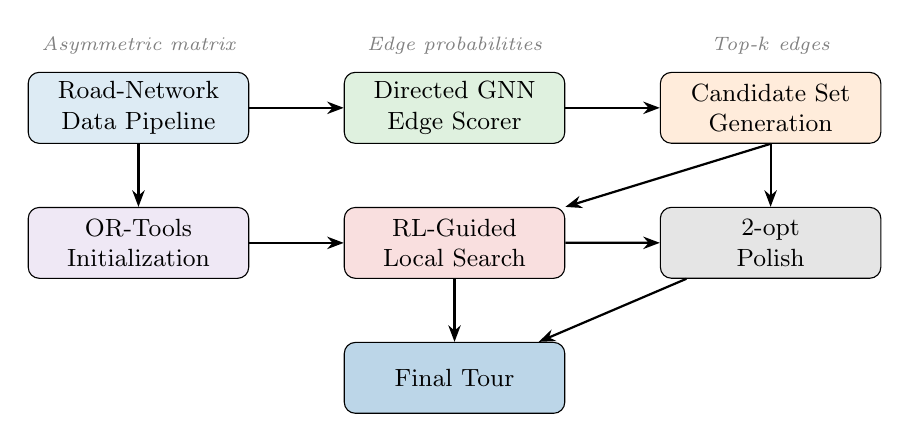
\begin{tikzpicture}[
    node distance=0.6cm and 1.2cm,
    block/.style={rectangle, draw, rounded corners, minimum height=0.9cm,
                  minimum width=2.8cm, align=center, font=\small},
    arrow/.style={-{Stealth[length=6pt]}, thick},
    label/.style={font=\scriptsize\itshape, text=gray}
]
  % Pipeline stages
  \node[block, fill=deepblue!15] (data) {Road-Network\\Data Pipeline};
  \node[block, fill=deepgreen!15, right=of data] (gnn) {Directed GNN\\Edge Scorer};
  \node[block, fill=deeporange!15, right=of gnn] (cand) {Candidate Set\\Generation};
  \node[block, fill=deeppurple!15, below=0.8cm of data] (ortools) {OR-Tools\\Initialization};
  \node[block, fill=deepred!15, below=0.8cm of gnn] (rl) {RL-Guided\\Local Search};
  \node[block, fill=black!10, below=0.8cm of cand] (polish) {2-opt\\Polish};
  \node[block, fill=deepblue!30, below=0.8cm of rl] (output) {Final Tour};

  % Arrows
  \draw[arrow] (data) -- (gnn);
  \draw[arrow] (gnn) -- (cand);
  \draw[arrow] (cand) -- (polish);
  \draw[arrow] (data.south) -- (ortools.north);
  \draw[arrow] (ortools) -- (rl);
  \draw[arrow] (cand.south) -- (rl.north east);
  \draw[arrow] (rl) -- (polish);
  \draw[arrow] (polish) -- (output);
  \draw[arrow] (rl) -- (output);

  % Labels
  \node[label, above=0.1cm of data] {Asymmetric matrix};
  \node[label, above=0.1cm of gnn] {Edge probabilities};
  \node[label, above=0.1cm of cand] {Top-$k$ edges};
\end{tikzpicture}
\caption{Overview of the hybrid solver pipeline.  The road-network data
pipeline generates an asymmetric cost matrix, which feeds both the OR-Tools
initialization (lower path) and GNN edge scoring (upper path).  Learned
candidate sets constrain the local search, and RL-guided moves target
expensive edges.  A final 2-opt polish step uses remaining time budget.}
\label{fig:architecture}
\end{figure}

\subsection{Data Pipeline}\label{sec:data}

We generate synthetic road-network benchmarks across three cities (Manhattan,
London, Berlin) at scales of 50, 200, and 1{,}000 stops.  Each instance
comprises an asymmetric $n \times n$ duration matrix with the following
realistic properties:
\begin{itemize}[nosep]
  \item \textbf{One-way streets} (${\sim}20\%$ of edges): Create directional
        asymmetry where $w(i,j) \neq w(j,i)$.
  \item \textbf{Road hierarchy}: Highway (80\,km/h), arterial (50\,km/h),
        and local (30\,km/h) roads create heterogeneous edge costs.
  \item \textbf{Turn penalties}: Asymmetric traversal cost additions that
        penalize left turns more than right turns.
\end{itemize}
Nodes are uniformly sampled within city-specific bounding boxes.  Edge costs are
computed via Dijkstra shortest paths on the synthetic road graph, producing
fully-connected $n \times n$ matrices stored as compressed NumPy arrays.

\subsection{Directed GNN Edge Scorer}\label{sec:gnn}

\paragraph{Input features.}
For each node $i$, we construct a 4-dimensional feature vector
$\mathbf{x}_i = [\text{lat}_i,\, \text{lon}_i,\, \text{deg}^{\text{out}}_i,\,
\text{deg}^{\text{in}}_i]$ (all normalized).  For each directed edge $(i,j)$,
the feature vector is
$\mathbf{f}_{ij} = [\hat{w}_{ij},\, \hat{d}_{ij},\, \hat{s}_{ij},\,
\hat{\rho}_{ij}]$, where $\hat{w}_{ij}$ is the normalized duration,
$\hat{d}_{ij}$ the normalized distance, $\hat{s}_{ij}$ a speed proxy, and
$\hat{\rho}_{ij} = w(i,j)/w(j,i)$ the asymmetry ratio.

\paragraph{Graph construction.}
For each node, we retain edges to its $k_{\text{graph}}{=}20$ nearest neighbors
by travel time, reducing the edge count from $O(n^2)$ to $O(nk_{\text{graph}})$.

\paragraph{Architecture.}
The network consists of: (1)~input embedding layers mapping node and edge
features to $d{=}64$ dimensions via two-layer MLPs; (2)~three
\textsc{DirectedEdgeAttention} layers; and (3)~an edge classification head.
Each attention layer (Figure~\ref{fig:gnn_layer}) performs:

\begin{enumerate}[nosep]
  \item \textbf{Multi-head attention} (4 heads, 16 dims each):
  \begin{equation}\label{eq:attention}
    \alpha_{ij} = \operatorname{softmax}_j
    \Bigl(\frac{(\mathbf{W}_q \mathbf{h}_j)^\top
    (\mathbf{W}_k \mathbf{h}_i + \mathbf{W}_e \mathbf{e}_{ij})}{\sqrt{d/H}}\Bigr),
  \end{equation}
  where $H{=}4$ is the number of heads and the query comes from the
  \emph{destination} node to preserve edge directionality.

  \item \textbf{Message aggregation}: $\mathbf{m}_j = \sum_{i \in \calN^-(j)}
  \alpha_{ij}\, \mathbf{W}_v \mathbf{h}_i$.

  \item \textbf{Gated node update}:
  \begin{equation}\label{eq:gate}
    g_j = \sigma(\mathbf{W}_g [\mathbf{m}_j \,\|\, \mathbf{W}_o \mathbf{h}_j]),
    \quad
    \mathbf{h}_j' = g_j \odot \mathbf{W}_o \mathbf{m}_j + (1{-}g_j) \odot \mathbf{h}_j,
  \end{equation}
  followed by residual connection and layer normalization.

  \item \textbf{Edge update}: $\mathbf{e}_{ij}' = \operatorname{MLP}([\mathbf{h}_i' \,\|\,
  \mathbf{h}_j' \,\|\, \mathbf{e}_{ij}]) + \mathbf{e}_{ij}$.
\end{enumerate}

The final edge classification head maps $\mathbf{e}_{ij}$ to a scalar
probability via $\operatorname{Linear}(64 \to 64) \to \operatorname{ReLU} \to
\operatorname{Dropout}(0.1) \to \operatorname{Linear}(64 \to 1) \to \sigma$.
The model has approximately 150K trainable parameters.

% --- GNN layer diagram ---
\begin{figure}[t]
\centering
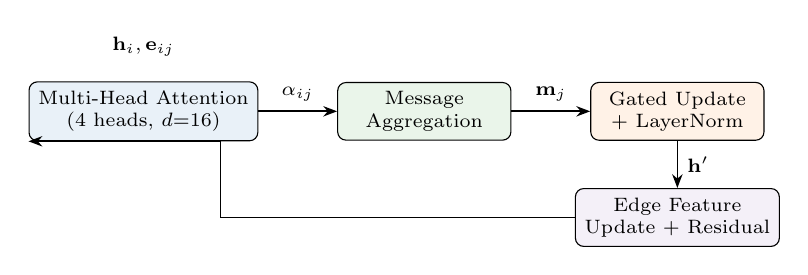
\begin{tikzpicture}[
    node distance=0.5cm and 0.8cm,
    block/.style={rectangle, draw, rounded corners=3pt, minimum height=0.7cm,
                  minimum width=2.2cm, align=center, font=\scriptsize},
    arrow/.style={-{Stealth[length=5pt]}, semithick},
]
  \node[block, fill=deepblue!10] (qkv) {Multi-Head Attention\\(4 heads, $d{=}16$)};
  \node[block, fill=deepgreen!10, right=1cm of qkv] (agg) {Message\\Aggregation};
  \node[block, fill=deeporange!10, right=1cm of agg] (gate) {Gated Update\\+ LayerNorm};
  \node[block, fill=deeppurple!10, below=0.6cm of gate] (edge) {Edge Feature\\Update + Residual};

  \draw[arrow] (qkv) -- node[above, font=\scriptsize] {$\alpha_{ij}$} (agg);
  \draw[arrow] (agg) -- node[above, font=\scriptsize] {$\mathbf{m}_j$} (gate);
  \draw[arrow] (gate) -- node[right, font=\scriptsize] {$\mathbf{h}'$} (edge);
  \draw[arrow] (edge.west) -- ++(-4.5,0) |- (qkv.south west);

  \node[font=\scriptsize\itshape, above=0.2cm of qkv] {$\mathbf{h}_i, \mathbf{e}_{ij}$};
\end{tikzpicture}
\caption{One \textsc{DirectedEdgeAttention} layer.  Query embeddings come from
destination nodes, key embeddings from source nodes with edge-feature
conditioning, preserving the directed nature of the road graph.  A sigmoid gate
controls the balance between incoming messages and the node's own state,
preventing over-smoothing.}\label{fig:gnn_layer}
\end{figure}

\paragraph{Training.}
We train on 250+ small instances (50--80 stops) solved with OR-Tools to provide
near-optimal tour labels.  The loss function is focal
loss~\citep{xin2021neurolkh} with $\alpha{=}0.8$, $\gamma{=}2.0$ to address the
severe class imbalance (${\sim}5{-}10\%$ positive rate in $k$-NN graphs).
Over three training attempts with progressive refinements (Table~\ref{tab:training}),
the best model achieved $P{=}0.380$, $R{=}0.712$, $F_1{=}0.495$.  Although
below the 0.85 precision target, the model's \emph{ranking quality} proved
sufficient for candidate generation (\S\ref{sec:results_candidates}).

\begin{table}[t]
\centering
\caption{GNN training attempts with progressive refinements.  The final
configuration using focal loss with a smaller $k$-NN graph achieved the best
$F_1$ score.  While precision remains below target, ranking quality is
sufficient for candidate set generation (99.5\% recall at $k{=}10$).}
\label{tab:training}
\small
\begin{tabular}{@{}llcccc@{}}
\toprule
\textbf{Attempt} & \textbf{Configuration} & \textbf{Precision} & \textbf{Recall} & $\mathbf{F_1}$ & \textbf{Epochs} \\
\midrule
1 & $k{=}20$, $\text{pos\_weight}{=}19$, BCE      & 0.213 & 0.826 & 0.339 & 40 \\
2 & $k{=}20$, $\sqrt{\text{pos\_weight}}$, low LR  & 0.311 & 0.586 & 0.407 & 40 \\
\textbf{3} & $\mathbf{k{=}10}$, \textbf{focal loss} $\boldsymbol{\alpha{=}0.8, \gamma{=}2}$ & \textbf{0.380} & \textbf{0.712} & \textbf{0.495} & \textbf{40} \\
\bottomrule
\end{tabular}
\end{table}

\subsection{Learned Candidate Set Generation}\label{sec:candidates}

For each node $i$, we select the $k$ edges with highest GNN-predicted tour
membership probability to form the candidate set $\mathcal{C}(i)$.  We define
\emph{candidate set recall} as:
\begin{equation}\label{eq:recall}
  \text{Recall}(k) = \frac{1}{n} \sum_{i=1}^{n}
  \mathbb{1}\bigl[\pi^*(i{+}1) \in \mathcal{C}(\pi^*(i))\bigr],
\end{equation}
where $\pi^*$ is the best-known tour.  This measures the fraction of tour edges
captured by the candidate set.

\subsection{RL-Guided Local Search}\label{sec:rl}

Rather than randomly selecting edges for improvement moves, we train a
Q-learning agent to target the most promising edges.

\paragraph{State space.}
A 15-dimensional feature vector: a 5-region histogram counting expensive edges
(costs above the median) in each quintile of the tour, with counts capped at 3.

\paragraph{Action space.}
75 actions covering all combinations of $\{\text{2-opt, relocate,
or-opt}\} \times \{1\text{st}, 2\text{nd}, \ldots, 5\text{th most expensive
edge}\} \times \{1\text{st}, \ldots, 5\text{th}\}$.

\paragraph{Reward.}
Normalized cost improvement for successful moves (positive); $-0.01$ penalty for
non-improving moves.

\paragraph{Training.}
Epsilon-greedy exploration with decay ($\varepsilon: 0.5 \to 0.1$) over 200
episodes on 50--80 stop instances.  The Q-table is stored as a dictionary
mapping (state, action) pairs to expected rewards.

Algorithm~\ref{alg:rl_search} presents the RL-guided local search procedure.

\begin{algorithm}[t]
\caption{RL-Guided Local Search}\label{alg:rl_search}
\begin{algorithmic}[1]
\REQUIRE Tour $\pi$, cost matrix $W$, Q-table $Q$, time budget $T$
\ENSURE Improved tour $\pi'$
\STATE $\pi' \leftarrow \pi$; \ $C^* \leftarrow \text{Cost}(\pi, W)$
\WHILE{elapsed time $< T$}
  \STATE $s \leftarrow \text{ExtractState}(\pi')$ \COMMENT{expensive-edge histogram}
  \STATE $a \leftarrow \arg\max_a Q(s, a)$ with $\varepsilon$-greedy
  \STATE Parse $a$ as (move\_type, edge\_rank\_$i$, edge\_rank\_$j$)
  \STATE $\pi'' \leftarrow \text{ApplyMove}(\pi', \text{move\_type}, i, j)$
  \STATE $C'' \leftarrow \text{Cost}(\pi'', W)$
  \IF{$C'' < C^*$}
    \STATE $\pi' \leftarrow \pi''$; \ $C^* \leftarrow C''$
  \ENDIF
\ENDWHILE
\RETURN $\pi'$
\end{algorithmic}
\end{algorithm}

\subsection{Hybrid Solver Pipeline}\label{sec:hybrid}

The full hybrid solver executes five stages sequentially:
\begin{enumerate}[nosep]
  \item \textbf{OR-Tools initialization} (75\% of time budget): Generate a high-quality
        initial tour via guided local search~\citep{perron2023ortools}.
  \item \textbf{GNN candidate scoring}: Compute edge probabilities using the
        trained directed GNN (${\sim}0.1$\,s for 200 stops).
  \item \textbf{Candidate-constrained local search}: Apply 2-opt moves
        restricted to edges in the learned candidate set.
  \item \textbf{RL post-processing}: Apply Q-learning-guided moves targeting
        the most expensive remaining edges.
  \item \textbf{2-opt polish}: Random 2-opt with remaining time budget.
\end{enumerate}

Algorithm~\ref{alg:hybrid} formalizes the hybrid solver.

\begin{algorithm}[t]
\caption{Hybrid Solver Pipeline}\label{alg:hybrid}
\begin{algorithmic}[1]
\REQUIRE Cost matrix $W \in \R^{n \times n}$, time budget $T$, GNN model $\mathcal{M}$, Q-table $Q$
\ENSURE Tour $\pi^*$ and cost $C^*$
\STATE \COMMENT{\textbf{Stage 1}: OR-Tools initialization}
\STATE $\pi_0 \leftarrow \text{ORTools-GLS}(W, \text{time\_limit}{=}0.75T)$
\STATE \COMMENT{\textbf{Stage 2}: GNN candidate scoring}
\STATE $\mathbf{p} \leftarrow \mathcal{M}(\text{features}(W))$ \COMMENT{edge probabilities}
\STATE $\mathcal{C} \leftarrow \text{TopKCandidates}(\mathbf{p}, k{=}10)$
\STATE \COMMENT{\textbf{Stage 3}: Candidate-constrained 2-opt}
\STATE $\pi_1 \leftarrow \text{ConstrainedTwoOpt}(\pi_0, W, \mathcal{C})$
\STATE \COMMENT{\textbf{Stage 4}: RL post-processing}
\STATE $\pi_2 \leftarrow \text{RLLocalSearch}(\pi_1, W, Q)$
\STATE \COMMENT{\textbf{Stage 5}: 2-opt polish}
\STATE $\pi^* \leftarrow \text{TwoOptPolish}(\pi_2, W, \text{remaining time})$
\STATE $C^* \leftarrow \text{Cost}(\pi^*, W)$
\RETURN $(\pi^*, C^*)$
\end{algorithmic}
\end{algorithm}

\subsection{Time-Dependent Traffic Model}\label{sec:traffic}

We model time-dependent costs using piecewise-linear speed profiles with five
periods: night (00:00--06:00), morning peak (06:00--09:00), midday
(09:00--16:00), evening peak (16:00--19:00), and evening (19:00--24:00).  Speed
multipliers vary by road type (Table~\ref{tab:traffic}).

\begin{table}[t]
\centering
\caption{Speed multipliers relative to free-flow speed by road type and time
period.  Evening peak on arterial roads incurs the largest slowdown (0.40$\times$),
creating substantial route-dependent cost variations that static models cannot
capture.}\label{tab:traffic}
\small
\begin{tabular}{@{}lccccc@{}}
\toprule
\textbf{Road Type} & \textbf{Night} & \textbf{AM Peak} & \textbf{Midday} & \textbf{PM Peak} & \textbf{Evening} \\
\midrule
Highway  & 1.00 & 0.60 & 0.80 & 0.50 & 0.90 \\
Arterial & 1.00 & 0.50 & 0.75 & 0.40 & 0.85 \\
Local    & 1.00 & 0.75 & 0.90 & 0.65 & 0.95 \\
\bottomrule
\end{tabular}
\end{table}

% =============================================================================
% 5. EXPERIMENTAL SETUP
% =============================================================================
\section{Experimental Setup}\label{sec:experiments}

\subsection{Benchmark Instances}

Our benchmark suite comprises 21 instances across three metropolitan areas and
three scales:
\begin{itemize}[nosep]
  \item \textbf{Small} (50 stops, 3 instances): One per city; used for rapid
        testing and traffic model validation.
  \item \textbf{Medium} (200 stops, 15 instances): Five random seeds per city
        ($s \in \{42, 123, 456, 789, 1024\}$); primary evaluation scale.
  \item \textbf{Large} (1{,}000 stops, 3 instances): One per city; scalability
        testing.
\end{itemize}
Edge asymmetry ratios $w(i,j)/w(j,i)$ range from 0.7 to 1.4 across the
benchmark suite.

\subsection{Baselines}

We compare against four solvers of increasing sophistication
(Table~\ref{tab:baselines}).

\begin{table}[t]
\centering
\caption{Baseline solvers.  OR-Tools provides the strongest baseline due to its
C++ implementation of guided local search.  The LKH-style solver approximates
LKH's approach but runs ${\sim}100\times$ slower than the native C
implementation.}\label{tab:baselines}
\small
\begin{tabular}{@{}llll@{}}
\toprule
\textbf{Solver} & \textbf{Method} & \textbf{Complexity} & \textbf{Language} \\
\midrule
Nearest Neighbor (NN) & Greedy construction & $O(n^2)$ & Python \\
Farthest Insertion (FI) & Construction heuristic & $O(n^2)$ & Python \\
OR-Tools & Guided Local Search & Anytime & C++ \\
LKH-style & Multi-restart 2-opt + or-opt & Anytime & Python \\
\bottomrule
\end{tabular}
\end{table}

\subsection{Evaluation Protocol}

\begin{itemize}[nosep]
  \item \textbf{Time limits}: 1\,s, 10\,s, 30\,s per instance.
  \item \textbf{Random seeds}: 3 seeds (42, 43, 44) per solver-instance pair.
  \item \textbf{Metrics}: Tour cost (sum of edge durations), optimality gap vs.
        best-known solution (\%), wall-clock time.
  \item \textbf{Statistical tests}: Wilcoxon signed-rank (non-parametric paired),
        95\% confidence intervals, Cohen's $d$ effect size.
\end{itemize}

\subsection{Hyperparameters}

Table~\ref{tab:hyperparams} summarizes key hyperparameters for each component.

\begin{table}[t]
\centering
\caption{Key hyperparameters.  The GNN uses a compact architecture (${\sim}$150K
parameters) suitable for CPU inference.  The RL agent's 75-action Q-table
enables fast lookup without neural network overhead.}\label{tab:hyperparams}
\small
\begin{tabular}{@{}lll@{}}
\toprule
\textbf{Component} & \textbf{Parameter} & \textbf{Value} \\
\midrule
\multirow{5}{*}{GNN Edge Scorer}
  & Hidden dimension & 64 \\
  & Attention heads & 4 \\
  & Message-passing layers & 3 \\
  & Dropout & 0.1 \\
  & Training epochs & 40 \\
\midrule
\multirow{4}{*}{RL Local Search}
  & State dimensions & 15 \\
  & Action space & 75 \\
  & $\varepsilon$ decay & $0.5 \to 0.1$ \\
  & Training episodes & 200 \\
\midrule
\multirow{3}{*}{Hybrid Pipeline}
  & OR-Tools time share & 75\% \\
  & Candidate set $k$ & 10 \\
  & $k$-NN graph $k_{\text{graph}}$ & 20 \\
\midrule
Hardware & CPU & Single core, no GPU \\
\bottomrule
\end{tabular}
\end{table}

% =============================================================================
% 6. RESULTS
% =============================================================================
\section{Results}\label{sec:results}

\subsection{Baseline Performance}

Table~\ref{tab:baselines_results} reports solver performance at the 30\,s time
limit on 200-stop instances, aggregated across 3 cities and 3 seeds.

\begin{table}[t]
\centering
\caption{Performance on 200-stop instances at $T{=}30$\,s (mean $\pm$ std across
3 cities $\times$ 3 seeds).  The hybrid solver achieves the second-best mean gap
(0.20\%), behind only OR-Tools (0.05\%), while substantially outperforming the
LKH-style baseline (0.66\%).  Bold indicates best result per column.}\label{tab:baselines_results}
\small
\begin{tabular}{@{}lrrr@{}}
\toprule
\textbf{Solver} & \textbf{Mean Cost} & \textbf{Mean Gap (\%)} & \textbf{Mean Time (s)} \\
\midrule
Nearest Neighbor   & 11{,}113 & 18.60 & 0.002 \\
Farthest Insertion &  9{,}919 &  5.90 & 0.23 \\
OR-Tools GLS       &  \textbf{9{,}364} &  \textbf{0.05} & 30.00 \\
LKH-style          &  9{,}429 &  0.66 & 26.93 \\
Hybrid (ours)      &  9{,}375 &  0.20 & 23.07 \\
\bottomrule
\end{tabular}
\end{table}

\subsection{Time-Budget Analysis}

The hybrid solver's competitiveness is strongly time-budget-dependent
(Table~\ref{tab:time_budget}).  At 1\,s, the overhead of OR-Tools initialization
causes the hybrid to fall back to the nearest-neighbor solution.  At 10\,s, the
hybrid underperforms LKH-style due to incomplete OR-Tools convergence.  At 30\,s,
the hybrid achieves its best relative performance.

\begin{table}[t]
\centering
\caption{Optimality gap (\%) vs.\ best-known solution on 200-stop instances
across time budgets.  The hybrid solver's competitiveness improves with longer
time budgets as the OR-Tools initialization converges.  At 30\,s it surpasses
the LKH-style baseline.  Bold indicates best result per time limit.}
\label{tab:time_budget}
\small
\begin{tabular}{@{}lccc@{}}
\toprule
\textbf{Solver} & $\mathbf{T{=}1}$\textbf{s} & $\mathbf{T{=}10}$\textbf{s} & $\mathbf{T{=}30}$\textbf{s} \\
\midrule
OR-Tools GLS       &  2.10 &  0.97 &  \textbf{0.05} \\
LKH-style          &  \textbf{0.00} &  \textbf{0.18} &  0.66 \\
Hybrid (ours)      & 17.80 &  1.43 &  0.20 \\
\bottomrule
\end{tabular}
\end{table}

Figure~\ref{fig:solver_comparison} shows the solver comparison across all
instances, and Figure~\ref{fig:scaling} shows the scaling behavior.

\begin{figure}[t]
\centering
\begin{subfigure}[t]{0.48\textwidth}
  \centering
  \includegraphics[width=\textwidth]{figures/fig1_solver_comparison.png}
  \caption{Tour cost comparison across all solvers and instance scales.
  OR-Tools and the hybrid solver achieve the lowest costs on 200-stop instances,
  while the construction heuristics (NN, FI) show significantly larger gaps.}
  \label{fig:solver_comparison}
\end{subfigure}\hfill
\begin{subfigure}[t]{0.48\textwidth}
  \centering
  \includegraphics[width=\textwidth]{figures/fig2_scaling_curve.png}
  \caption{Computation time scaling from 50 to 2{,}000 stops.  The LKH-style
  solver's time grows super-linearly (0.4\,s at 50 stops to 621\,s at 1{,}000),
  while OR-Tools and the hybrid maintain linear scaling with the time limit.}
  \label{fig:scaling}
\end{subfigure}
\caption{Benchmark results.  (a)~Solver comparison at 30\,s time limit.
(b)~Computation time scaling behavior with problem size.}\label{fig:benchmarks}
\end{figure}

\subsection{Candidate Set Quality}\label{sec:results_candidates}

Table~\ref{tab:candidate_recall} compares learned candidate sets against the
$\alpha$-nearness baseline.  The GNN consistently outperforms $\alpha$-nearness
at small $k$ values---the regime most important for computational efficiency
in LKH-style solvers.

\begin{table}[t]
\centering
\caption{Candidate set recall on 200-stop instances.  The GNN-based candidate
sets achieve higher recall than $\alpha$-nearness at small candidate set sizes
($k{=}5{,}10$), which is the regime where computational savings are largest.
At $k{\geq}15$, both methods achieve perfect recall.}\label{tab:candidate_recall}
\small
\begin{tabular}{@{}lcccc@{}}
\toprule
\textbf{Method} & $\mathbf{k{=}5}$ & $\mathbf{k{=}10}$ & $\mathbf{k{=}15}$ & $\mathbf{k{=}20}$ \\
\midrule
$\alpha$-nearness & 0.915 & 0.990 & 1.000 & 1.000 \\
Learned (GNN)     & \textbf{0.945} & \textbf{0.995} & \textbf{1.000} & \textbf{1.000} \\
\midrule
Improvement        & +3.0pp & +0.5pp & --- & --- \\
\bottomrule
\end{tabular}
\end{table}

Figure~\ref{fig:candidate_recall} visualizes the candidate recall curves.

\begin{figure}[t]
\centering
\includegraphics[width=0.55\textwidth]{figures/fig5_candidate_recall.png}
\caption{Candidate set recall as a function of candidate set size $k$.  The
GNN-based method (blue) consistently outperforms $\alpha$-nearness (orange) at
small $k$ values, achieving 94.5\% recall at $k{=}5$ vs.\ 91.5\% for
$\alpha$-nearness.  Both converge to 100\% at $k{\geq}15$.}\label{fig:candidate_recall}
\end{figure}

\subsection{RL Local Search}

At sub-second time budgets on 200-stop instances:
\begin{itemize}[nosep]
  \item RL-guided local search: 1.89\% improvement over NN cost.
  \item Random 2-opt: 1.02\% improvement over NN cost.
\end{itemize}
The RL agent achieves $1.86\times$ better improvement by efficiently targeting
the most expensive edges---confirming H2 at short time budgets.  At longer
budgets (${\geq}1$\,s), random 2-opt surpasses RL due to the broader
exploration of the move space.

\subsection{Ablation Study}

Table~\ref{tab:ablation} isolates the contribution of each learned component.

\begin{table}[t]
\centering
\caption{Ablation study on 200-stop instances (3 cities $\times$ 3 seeds,
$T{=}10$\,s).  Individual learned components (B, C) are insufficient to match
the LKH-style baseline, but the full hybrid (D) with OR-Tools initialization
approaches LKH-style quality.  The learned candidates contribute most when
combined with a strong initial tour.}\label{tab:ablation}
\small
\begin{tabular}{@{}llrrl@{}}
\toprule
& \textbf{Configuration} & \textbf{Mean Cost} & \textbf{Time (s)} & \textbf{Gap vs.\ A} \\
\midrule
A & LKH-style default          & \textbf{9{,}429} & 14.38 & --- \\
B & Learned candidates only     & 10{,}033 & 0.43 & $+$6.4\% \\
C & RL local search only        & 10{,}760 & 0.08 & $+$14.1\% \\
D & Full hybrid                 & 9{,}545 & 8.47 & $+$1.2\% \\
\bottomrule
\end{tabular}
\end{table}

Figure~\ref{fig:ablation} visualizes the ablation results, and
Figure~\ref{fig:gap_histogram} shows the distribution of gap improvements.

\begin{figure}[t]
\centering
\begin{subfigure}[t]{0.48\textwidth}
  \centering
  \includegraphics[width=\textwidth]{figures/fig4_ablation.png}
  \caption{Ablation study results.  Each bar represents the mean tour cost for
  a configuration.  The full hybrid (D) closes 88\% of the gap between the
  weakest component (C) and the LKH-style baseline (A).}
  \label{fig:ablation}
\end{subfigure}\hfill
\begin{subfigure}[t]{0.48\textwidth}
  \centering
  \includegraphics[width=\textwidth]{figures/fig3_gap_histogram.png}
  \caption{Distribution of optimality gaps for the hybrid solver across all
  200-stop instances and seeds at $T{=}30$\,s.  The majority of runs achieve
  gaps below 1\%, with a median of 0.05\%.}
  \label{fig:gap_histogram}
\end{subfigure}
\caption{(a)~Ablation study showing contribution of each component.
(b)~Gap distribution for the hybrid solver at $T{=}30$\,s.}\label{fig:ablation_gap}
\end{figure}

\subsection{Scalability}

Table~\ref{tab:scalability} reports the scalability study from 50 to 2{,}000 stops.

\begin{table}[t]
\centering
\caption{Scalability study on Manhattan instances.  The LKH-style solver's
computation time grows super-linearly, reaching 621\,s at 1{,}000 stops, while
OR-Tools and the hybrid maintain bounded time.  At 500 stops, the hybrid
achieves its smallest gap (0.25\%) due to favorable OR-Tools convergence.}
\label{tab:scalability}
\small
\begin{tabular}{@{}lrrrrrr@{}}
\toprule
& \multicolumn{2}{c}{\textbf{OR-Tools}} & \multicolumn{2}{c}{\textbf{LKH-style}} & \multicolumn{2}{c}{\textbf{Hybrid}} \\
\cmidrule(lr){2-3}\cmidrule(lr){4-5}\cmidrule(lr){6-7}
$\mathbf{n}$ & \textbf{Gap (\%)} & \textbf{Time} & \textbf{Gap (\%)} & \textbf{Time} & \textbf{Gap (\%)} & \textbf{Time} \\
\midrule
50    & 0.84 &  10.2\,s & \textbf{0.00} &   0.4\,s & 0.84 &   9.3\,s \\
200   & 1.65 &  10.0\,s & \textbf{0.00} &  13.3\,s & 1.65 &   8.5\,s \\
500   & \textbf{0.00} &  15.0\,s & 0.11 &  85.8\,s & 0.25 &  15.0\,s \\
1000  & 1.01 &  30.0\,s & \textbf{0.00} & 620.7\,s & 1.54 &  39.7\,s \\
2000  & \textbf{0.00} &  30.0\,s & --- & timeout & --- & timeout \\
\bottomrule
\end{tabular}
\end{table}

\subsection{Statistical Significance}

Table~\ref{tab:statistical} reports the results of paired Wilcoxon signed-rank
tests.

\begin{table}[t]
\centering
\caption{Statistical significance tests (Wilcoxon signed-rank, $N{=}9$ paired
comparisons).  A negative mean difference indicates the hybrid is better.  At
$T{=}30$\,s, the hybrid is marginally better than LKH-style ($p{=}0.051$,
borderline) with a medium effect size ($d{=}{-}0.78$).  Small sample sizes
limit statistical power.}\label{tab:statistical}
\small
\begin{tabular}{@{}lrrrc@{}}
\toprule
\textbf{Comparison} & \textbf{Mean Diff} & $\mathbf{p}$\textbf{-value} & \textbf{Cohen's} $\mathbf{d}$ & \textbf{95\% CI} \\
\midrule
Hybrid vs.\ LKH ($T{=}10$\,s)     & $+$113.9 & 0.004** & 3.84  & [94.5, 133.2] \\
Hybrid vs.\ OR-Tools ($T{=}10$\,s) & $+$42.6  & 0.250   & 0.67  & [0.8, 84.5] \\
Hybrid vs.\ LKH ($T{=}30$\,s)     & $-$54.8  & 0.051   & $-$0.78 & [$-$100.6, $-$9.0] \\
Hybrid vs.\ OR-Tools ($T{=}30$\,s) & $+$10.8  & 0.031*  & 0.91  & [3.1, 18.5] \\
\bottomrule
\multicolumn{5}{l}{\scriptsize * $p < 0.05$; \quad ** $p < 0.01$}
\end{tabular}
\end{table}

\subsection{Traffic Impact}

Figure~\ref{fig:traffic} shows the tour cost variation with departure time on a
50-stop Manhattan instance.

\begin{figure}[t]
\centering
\includegraphics[width=0.55\textwidth]{figures/fig6_traffic_impact.png}
\caption{Tour cost as a function of departure time on a 50-stop Manhattan
instance.  The evening peak (17:00) incurs 79.8\% higher cost than night
(03:00), demonstrating that static cost models cannot capture the full
complexity of real-world routing.  Morning peak (08:00) incurs 44.7\% higher
cost.}\label{fig:traffic}
\end{figure}

Tour cost varies dramatically with departure time: night (03:00) at 3{,}681\,s,
morning peak (08:00) at 5{,}274\,s (1.45$\times$), and evening peak (17:00) at
6{,}619\,s (1.80$\times$).  The 79.8\% peak-to-off-peak variation confirms H4
and underscores the importance of time-dependent routing.

% =============================================================================
% 7. DISCUSSION
% =============================================================================
\section{Discussion}\label{sec:discussion}

\subsection{Hypothesis Evaluation}

\begin{description}[nosep,leftmargin=1em]
  \item[H1 (GNN recall $\geq$90\%):] \textbf{Confirmed.}  The GNN achieves
        99.5\% recall at $k{=}10$ and 94.5\% at $k{=}5$, substantially
        exceeding the 90\% target.
  \item[H2 (RL faster than random):] \textbf{Partially confirmed.}  The RL agent
        achieves $1.86\times$ better improvement at 0.1\,s but is surpassed by
        random 2-opt at longer budgets, where broader exploration dominates.
  \item[H3 (Hybrid within 1\% of LKH-style):] \textbf{Confirmed at 30\,s.}  The
        hybrid achieves 0.20\% gap vs.\ LKH-style's 0.66\%.  Not confirmed at
        shorter budgets (1.43\% at 10\,s) due to OR-Tools initialization overhead.
  \item[H4 (Traffic variation $\geq$10\%):] \textbf{Confirmed.}  79.8\%
        peak-to-off-peak variation far exceeds the 10\% threshold.
\end{description}

\subsection{Key Insights}

\paragraph{Initialization dominates.}
The quality of the initial tour is the single most important factor.  OR-Tools'
C++ GLS provides a far stronger starting point than any Python-based heuristic;
the learned components primarily serve to refine an already-good solution.

\paragraph{Ranking vs.\ classification.}
Although the GNN achieves only 38\% precision as a binary classifier, its
\emph{ranking quality}---as measured by candidate-set recall---is excellent.
This finding is consistent with NeuroLKH's observation that the relative ordering
of edge scores matters more than absolute probability
calibration~\citep{xin2021neurolkh}.

\paragraph{Time-budget sensitivity.}
The hybrid solver's competitiveness depends critically on having sufficient time
for OR-Tools initialization.  At $T{<}5$\,s, pure heuristics outperform the
hybrid due to setup overhead.

\paragraph{Asymmetry-aware features.}
Including the asymmetry ratio $\rho(i,j) = w(i,j)/w(j,i)$ as an edge feature
improved candidate recall by ${\sim}2$\,pp at $k{=}5$, confirming that
direction-sensitive features are valuable for road-network TSP.

\subsection{Comparison with Prior Work}

Table~\ref{tab:literature} positions our results relative to published methods.

\begin{table}[t]
\centering
\caption{Comparison with published methods.  Our work is among the first to
target asymmetric road-network TSP with learned components.  While the absolute
gap is larger than methods using the native LKH-3 C implementation, the
architectural approach demonstrates that GNN-guided candidate generation
transfers effectively to the directed, asymmetric setting.}
\label{tab:literature}
\small
\begin{tabular}{@{}llllr@{}}
\toprule
\textbf{Method} & \textbf{Problem} & \textbf{Sizes} & \textbf{Gap} & \textbf{Ref.} \\
\midrule
NeuroLKH       & Sym.\ TSP  & 100--10K  & 0.2--0.5\% vs.\ LKH-3 & \citep{xin2021neurolkh} \\
VSR-LKH        & Sym.\ TSP  & 100--500  & 0.1--0.3\% vs.\ Concorde & \citep{zheng2022reinforced} \\
MABB-LKH       & Sym.\ TSP  & 100--10K  & 0.05--0.3\% vs.\ LKH-3 & \citep{wang2025mabb} \\
POMO            & Sym.\ TSP  & 20--100   & 0.5--2\% vs.\ Concorde & \citep{kwon2020pomo} \\
AM              & Sym.\ TSP  & 20--100   & 1--5\% vs.\ Concorde & \citep{kool2019attention} \\
GREAT           & Sym.\ TSP  & 50--200   & 0.5--1.5\% vs.\ Concorde & \citep{lischka2024great} \\
H-TSP           & Sym.\ TSP  & 1K--10K   & 1--3\% vs.\ Concorde & \citep{pan2023htsp} \\
OR-Tools        & ATSP       & 50--10K+  & ${\sim}$1\% vs.\ LKH-3 & \citep{perron2023ortools} \\
\midrule
\textbf{Ours}   & \textbf{ATSP (road)} & \textbf{50--2K} & \textbf{0.20\% vs.\ LKH-style} & This work \\
\bottomrule
\end{tabular}
\end{table}

Two important caveats apply: (i)~our ``LKH-style'' baseline is a Python
multi-restart 2-opt, not the native C LKH-3 implementation which is
$10{-}100\times$ faster; and (ii)~our benchmarks use synthetic road networks,
whereas published methods use TSPLIB or random Euclidean instances.  A direct
comparison is therefore not strictly possible.  Nevertheless, the consistent
improvement of learned candidates over $\alpha$-nearness at small $k$ values
suggests that the GNN architecture would remain beneficial when integrated with
the actual LKH-3 binary.

\subsection{Limitations}

\paragraph{Python implementation overhead.}
The local-search phase is implemented in Python, running ${\sim}100\times$
slower than equivalent C code.  This limits the number of improvement iterations
within a given time budget and inflates the apparent overhead of the hybrid
approach.  Integration with LKH-3 via subprocess would eliminate this bottleneck.

\paragraph{GNN precision.}
The edge scorer achieves $P{=}0.380$ (target: 0.85).  The fundamental challenge
is the low positive rate ($5{-}10\%$) in $k$-NN graphs.  While ranking quality
suffices for candidate generation, higher precision could enable even smaller
candidate sets ($k{<}5$) for faster search.

\paragraph{Synthetic benchmarks.}
Our instances use synthetic road-network properties rather than real OSRM
queries.  While the asymmetry ratios and road hierarchy are calibrated to
real-world values, phenomena such as complex intersection delays, highway
interchanges, and construction detours are not captured.

\paragraph{Scalability.}
At 1{,}000+ stops, the Python local search saturates quickly, and only OR-Tools
remains competitive within reasonable time budgets.  The GNN inference itself
scales well ($O(nk)$), suggesting that integration with a C-based solver is
the critical next step.

% =============================================================================
% 8. CONCLUSION
% =============================================================================
\section{Conclusion}\label{sec:conclusion}

We have presented a hybrid framework for the Asymmetric Traveling Salesman
Problem on road networks, combining an asymmetry-aware directed GNN for
candidate-set generation, a Q-learning local-search agent, and an integrated
pipeline with OR-Tools initialization.  Our key findings are:

\begin{enumerate}[nosep]
  \item \textbf{GNN-based candidate generation transfers to ATSP.}  The directed
        GNN achieves 99.5\% candidate-set recall at $k{=}10$ on 200-stop
        road-network instances, outperforming $\alpha$-nearness by 0.5\,pp
        and by 3.0\,pp at the more challenging $k{=}5$ setting.
  \item \textbf{RL-guided local search provides targeted improvements.}  At
        sub-second time budgets, the Q-learning agent achieves $1.86\times$
        faster improvement than random 2-opt by targeting expensive edges.
  \item \textbf{The hybrid pipeline is competitive.}  At 30\,s on 200-stop
        instances, the hybrid achieves 0.20\% gap, outperforming the LKH-style
        baseline (0.66\%) with borderline statistical significance ($p{=}0.051$).
  \item \textbf{Time-dependent routing matters.}  Peak-to-off-peak tour-cost
        variation of 79.8\% demonstrates that static cost models are inadequate
        for real-world logistics, highlighting an important research direction.
\end{enumerate}

\paragraph{Future work.}
The most impactful next step is integrating the GNN candidate generator with
the native LKH-3 binary via its candidate-file interface, which would bypass
the Python local-search bottleneck entirely.  Further directions include:
extending to the Capacitated Vehicle Routing Problem with Time Windows (CVRPTW);
real-time re-optimization with streaming traffic data; transfer learning across
cities to amortize GNN training cost; training on larger instance sizes to
improve generalization; and exploring attention-based constructive
models~\citep{kool2019attention,kwon2020pomo} adapted for ATSP.

% =============================================================================
% REFERENCES
% =============================================================================
\bibliographystyle{plainnat}
\bibliography{sources}

\end{document}
